% !Mode::"TeX:UTF-8"
\documentclass[a4paper]{article}
\usepackage{amssymb}
\usepackage{geometry}
\usepackage{graphicx}
\usepackage{fancyhdr}
\usepackage{setspace}
\usepackage{pdfpages}
\usepackage{listings}
\usepackage{amsthm}
\usepackage{url}
\usepackage{hyperref}
\usepackage{subcaption}

\graphicspath{{./figure/}}

\geometry{left=2.5cm,right=2.5cm,top=2.5cm,bottom=2.5cm}

\author{Chi Zhang\\\\USC ID: 6099-4134-05\\\\Department of Computer Science\\\\University of Southern California}
\title{CSCI 699 Spring 2019\\Machine Learning for Knowledge Extraction \& Reasoning\\Homework 2\thanks{Instructor: Xiang Ren}}

\begin{document}

  \maketitle                     %generate the title
  \begin{spacing}{1.0}
 
  \section{Code Repository}
  \url{https://github.com/vermouth1992/CSCI699ml4know/tree/master/hw2}
 
  \section{Development Pipeline}
  We started from an open source implementation of CNN for relation extraction \cite{re_cnn} from \url{https://github.com/ShomyLiu/pytorch-pcnn} and try various ideas to improve the results. For model architecture, we tried CNN with multi-sized window kernel \cite{pcnn} and RNN with attention \cite{Zhou2016AttentionBasedBL}. We also tried CNN with rank loss \cite{cnn_rank_loss}. Some ideas are inspired by a great blog of various models for relation extraction in \url{http://shomy.top/2018/02/28/relation-extraction/}.

   
  \subsection{Features}
  We consider lexical features as described in \cite{re_cnn}: entity1, entity2, and the left and right token of the two entities. We don't use hypernyms in WordNet since it is from extra source. For sentence level feature, we consider word embedding and position features. We use pre-trained word embedding from Glove \cite{glove} with 50 dimension to initialize our embedding layer. The position feature measures the distance of each word to the two entities. The distance index will be passed to an embedding layer as well.
  
  We use open source nltk tokenizer (\url{https://www.nltk.org}) for tokenization of raw sentences. 
  
  \subsection{Model Architecture}
  \begin{figure}
    \centering
    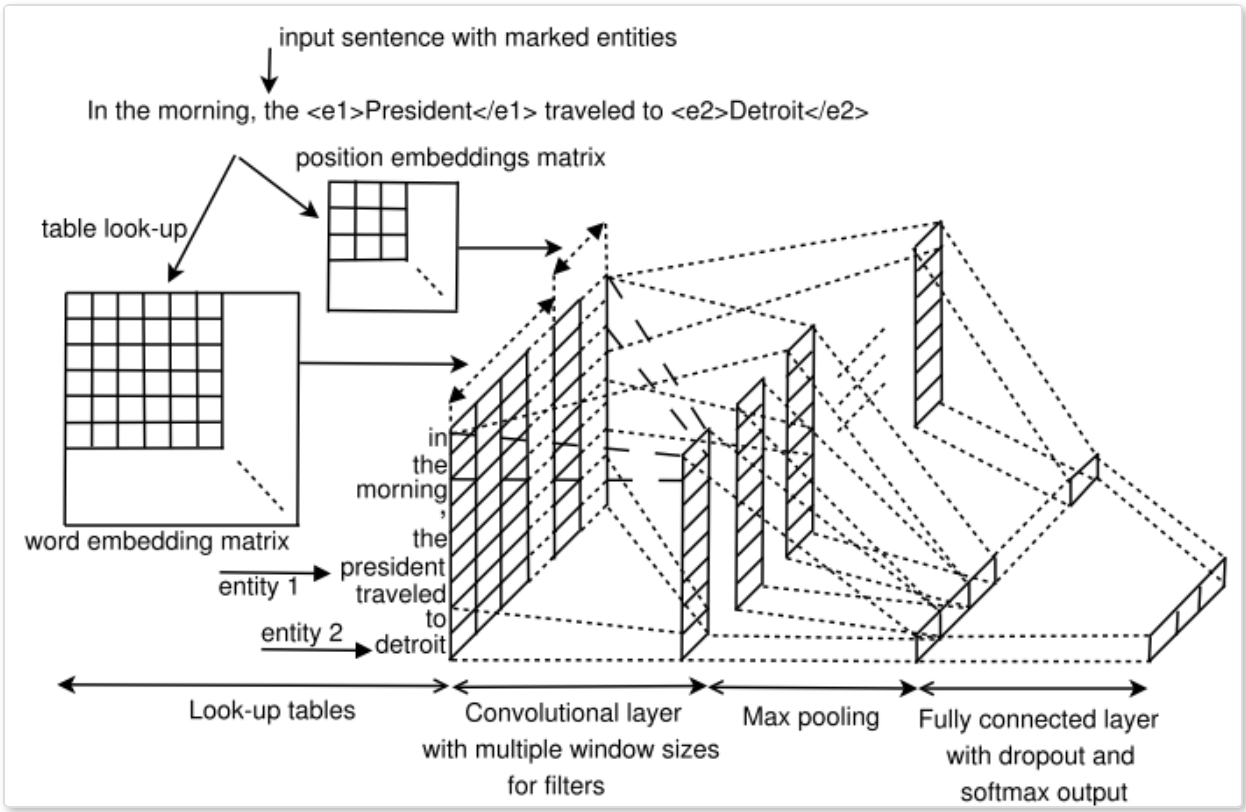
\includegraphics[width=\linewidth]{cnn_multi_window}
    \caption{CNN architecture for relation extraction with multi-sized window \cite{pcnn}}
    \label{fig:cnn_multi_window}
  \end{figure}
  For CNN-based model, we consider PCNN as described in \cite{pcnn} as shown in Figure~\ref{fig:cnn_multi_window}. Compared with single-sized window kernel in \cite{re_cnn}, multi-sized kernel is able to capture multiple n-gram features.
  
  \begin{figure}
    \centering
    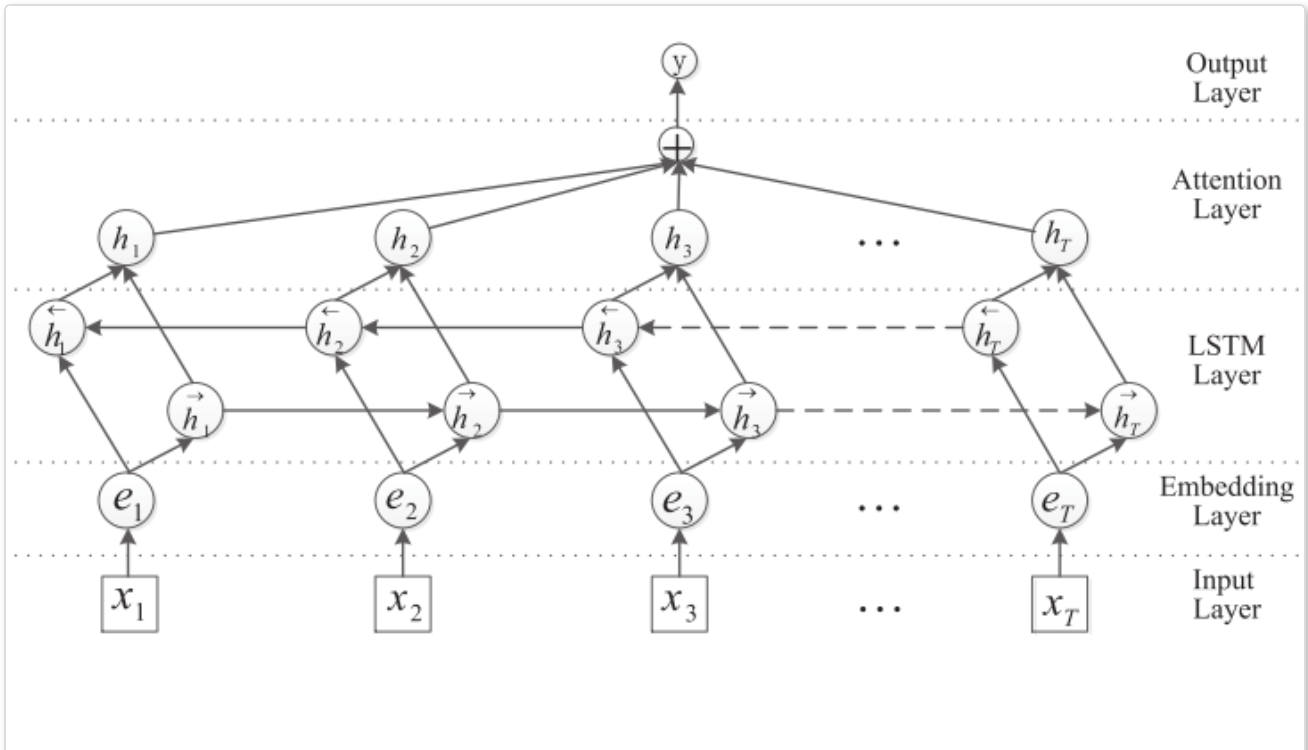
\includegraphics[width=\linewidth]{rnn_attention}
    \caption{RNN architecture for relation extraction with attention \cite{Zhou2016AttentionBasedBL}}
    \label{fig:rnn_attention}
  \end{figure}
  For RNN-based model, we consider standard BiLSTM with output attention in \cite{Zhou2016AttentionBasedBL} and the architecture is shown in Figure~\ref{fig:rnn_attention}. In this model, we only use sentence feature with word embedding and position embedding. The attention layer takes a weight sum of the output of BiLSTM layer. Assume $H=[h_1,h_2,\cdots, h_T]$, then the weighted sum is calculated as 
  \begin{equation}
  M=\tanh(H)
  \end{equation}
  \begin{equation}
  \alpha=softmax(w^TM)
  \end{equation}
  \begin{equation}
  r=H\alpha^T
  \end{equation}
  where $\alpha$ is the attention weights.
  
  \subsection{Loss Function}
  There is one problem using raw cross entropy loss. The "Other" class is treated the same as other classes. This is problematic because "Other" class contains more redundant distribution than normal classes. In \cite{cnn_rank_loss}, the author proposes rank loss defined as 
  \begin{equation}
  L=\log(1+\exp(\gamma(m^{+}-s_{\theta}(x)_{y^+}))) + \log(1+\exp(\gamma(m^{-}+s_{\theta}(x)_{y^-})))
  \end{equation}
  where $s$ is the final score for class $y+$ and $y-$. The negative label used is the one with maximum score. $m$ is a margin to separate positive and negative scores. We treat ``Other" labels separately. During training, we set $s_{\theta}(x)_{y^+}$ to be zero directly. During testing, if all the score are less than zero, we classify it as ``Other".
  
  \section{Performance Analysis}
  During experiments, we randomly choose 800 examples for validation. All the models are trained in 100 epoch and pick the one with greatest validation F1 score. 
  
  \subsection{Compare various window-size for CNN}
  \begin{table}
    \centering
    \caption{Performance of CNN model with various window-size}
    \begin{tabular}{|c|c|}
      \hline
      Window size & F1 score \\\hline
      3        &  80.75\% \\\hline
      2, 3, 4, 5 & 82.01\% \\\hline
      2, 3, 4, 5, 6, 7, 8 & 82.25\% \\\hline
      2, 3, 4, 5, 6, 7, 8, 9, 10, 11, 12 & 82.17\% \\\hline
    \end{tabular}
    \label{tab:cnn_window_size}
  \end{table}
  We show the F1 score with various window-size in Table~\ref{tab:cnn_window_size}. By using multi-size window size, the F1 performance increases around 1.5\%. However, keep increasing the window size will cause the model to overfitting. In the following experiments, we use window size of $[2, 3, 4, 5, 6, 7, 8]$.
  
  \subsection{The effect of rank loss for CNN-based model}
  We train the model with rank loss \cite{cnn_rank_loss} and the multi-sized window is $[2, 3, 4, 5, 6, 7, 8]$. The final F1 score is $82.89\%$, which increases by $0.64\%$.
  
  \subsection{RNN model with attention}
  Finally, we train RNN model with attention. The validation F1 score is $82.25\%$, which is compared to CNN-based model. However, we didn't use lexical features in RNN-based model.  
  
  
  \end{spacing}  
  \bibliographystyle{abbrv}
  \bibliography{./bib/chizhang.bib}

\end{document}
